\documentclass[10pt]{article}
\usepackage{icmlko}

\icmlmeta{IP 파운데이션 월드모델}{45}{배선도 바닥났다}{후보 오십 개 중 문턱을 넘는 것이 없다 --- 그리고 알고리즘을 검정하려면 표본이 서른 배 필요하다}

\begin{document}

\twocolumn[
\icmlheader

\begin{abstract}
노트 44는 지렛대를 둘로 좁혔다 --- 배선과 데이터. 배선은 효과가 크고
(노트 34의 $+$0.0939, 구간 {[}$+$0.046, $+$0.199{]}) 검정도 싸므로 먼저 훑었다.
다섯 도메인의 슬롯별 후보 \textbf{오십 개}를 스무 셀 평균 순위 상관으로 전수
검정했다. \textbf{문턱(0.02)을 넘는 것이 하나도 없다.} 최대가 게임 타깃 폭을
지원 언어 수로 바꾸는 $+$0.0134이고, 나머지 마흔아홉은 그 아래다. 현재 배선이
후보 공간 안에서 지역 최적이라는 뜻이며, \textbf{노트 44가 남긴 두 지렛대 중
하나가 소진됐다.} 그러면 데이터를 얼마나 늘려야 하는지가 다음 질문이다.
부분추출로 구간 반폭이 표본에 어떻게 의존하는지 쟀다. 679건에서 0.186,
1,241건(현재)에서 0.061로 단조 감소한다. 보수적으로 $n^{-1/2}$를 가정하면
배선 급 효과(0.094)를 확실히 보려면 \textbf{1.7배}, 공통 축 급(0.022)은
\textbf{31배}, 이중 배선 급(0.009)은 \textbf{186배}가 필요하다. 측정된 기울기
($-$1.77)로 외삽하면 각각 1.2배, 2.7배, 4.5배다. 어느 쪽이든 결론은 같다 ---
\textbf{배선 급 효과는 지금도 볼 수 있고 알고리즘 급 효과는 볼 수 없다.}
그리고 구간을 좁히는 가장 싼 길은 레코드가 아니라 \emph{도메인}이다. 도메인이
하나 늘면 셀이 20개에서 30개로 늘어 평균 자체가 안정된다.
\end{abstract}
]

\section{배선을 전수로 훑는다}

노트 38도 배선을 탐색했지만 목적함수가 인자 공간 자기 상관이었고 그것은 MAE
계열이라 눈금에 반응한다(노트 42). 여기서는 스무 셀 평균 순위 상관을 직접
목적으로 쓴다.

두 단계로 나눴다. 후보마다 붓스트랩 300회를 돌리면 계산이 감당이 안 된다.

\begin{itemize}[leftmargin=1.1em,itemsep=0.15em]
\item \textbf{1단계} --- 후보 오십 개의 점추정 $\Delta\rho$. 한 후보에 한 번씩.
\item \textbf{2단계} --- $|\Delta\rho|\ge0.02$인 것만 짝지은 붓스트랩. 문턱은
      노트 44에서 왔다 --- 알고리즘 조정 셋의 효과가 0.009--0.022였고 전부
      구간이 0을 포함했으므로 그 아래는 볼 필요가 없다.
\end{itemize}

\begin{figure}[t]
\centering
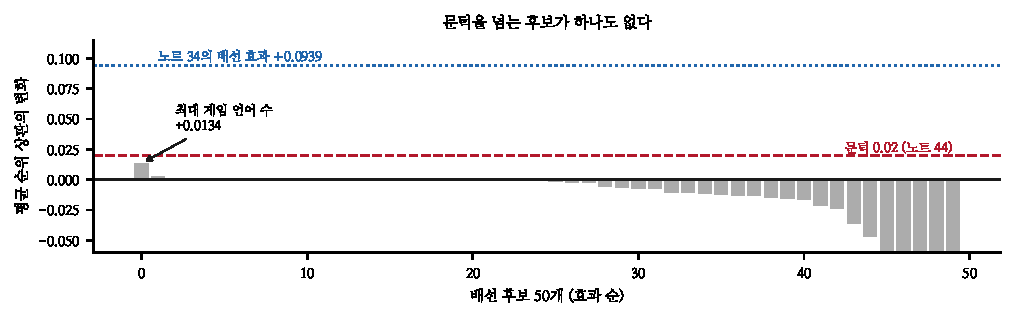
\includegraphics[width=\textwidth]{figs/exhaust.pdf}
\caption{배선 후보 오십 개의 효과. 점선이 문턱, 위 점선이 노트 34의 효과다.}
\end{figure}

\begin{table}[t]
\centering\tsize
\caption{상위 후보. 현행 평균 $\rho=+0.3516$.}
\begin{tabular}{lllr}
\toprule
도메인 & 슬롯 & 후보 & $\Delta\rho$ \\
\midrule
게임 & 타깃 폭 & 지원 언어 수 & \textbf{$+$0.0134} \\
게임 & 굿즈 규모 & 설치 용량 & $+$0.0025 \\
\multicolumn{3}{l}{나머지 48개} & $\le+0.0000$ \\
\bottomrule
\end{tabular}
\end{table}

\claimx{현재 배선은 관측 가능한 후보 공간 안에서 지역 최적이다. 오십 개 중
문턱을 넘는 것이 없고 최대가 $+$0.0134다.}{새 변수를 수집하면 후보 공간이
커지므로 이 결론은 ``지금 가진 변수로는''이라는 조건 아래에서만 참이다.}

2단계는 돌릴 것이 없었다. \textbf{노트 44가 남긴 두 지렛대 중 하나가 소진됐다.}

\section{그러면 데이터가 얼마나 필요한가}

부분추출로 구간 반폭이 표본에 어떻게 의존하는지 쟀다. 도메인마다 연도 층화
비복원 추출로 줄이고, 각 크기에서 붓스트랩 200회로 구간을 구한다.

\begin{table}[t]
\centering\tsize
\caption{표본과 구간 반폭.}
\begin{tabular}{rrrr}
\toprule
비율 & 레코드 & 반폭 & 평균 $\rho$ \\
\midrule
0.20 & 679 & 0.1857 & $+$0.2471 \\
0.30 & 740 & 0.1457 & $+$0.2576 \\
0.45 & 830 & 0.0887 & $+$0.3736 \\
0.60 & 927 & 0.0819 & $+$0.3199 \\
0.80 & 1,112 & 0.0680 & $+$0.3345 \\
1.00 & \textbf{1,241} & \textbf{0.0614} & $+$0.3320 \\
\bottomrule
\end{tabular}
\end{table}

\begin{figure}[t]
\centering

\includegraphics[width=\textwidth]{figs/power.pdf}
\caption{로그-로그. 두 외삽선 사이가 실제 필요량이다.}
\end{figure}

측정된 기울기는 $-$1.77인데 부분추출 폭이 좁아(679--1,241) 믿기 어렵다.
$n^{-1/2}$를 보수 하한으로 두고 둘 다 적는다.

\begin{table}[t]
\centering\tsize
\caption{효과를 구간 밖으로 밀어내는 데 필요한 레코드.}
\begin{tabular}{lrrr}
\toprule
보려는 효과 & 필요 반폭 & 보수 & 적합 \\
\midrule
배선 급 (0.094) & 0.047 & \textbf{1.7배} & 1.2배 \\
공통 축 급 (0.022) & 0.011 & 31배 & 2.7배 \\
이중 배선 급 (0.009) & 0.0045 & 186배 & 4.5배 \\
\bottomrule
\end{tabular}
\end{table}

\claimx{배선 급 효과(0.09)는 현재 표본의 1.2--1.7배면 확실히 보이고, 알고리즘
급 효과(0.01--0.02)는 3--30배가 필요하다. 후자는 실질적으로 검정 불가능한
영역이다.}{도메인을 늘려 셀 수가 제곱으로 증가하면 필요량이 이 계산보다 훨씬
줄 수 있다. 그 경우 보수 외삽이 지나치게 비관적인 것이다.}

\paragraph{레코드보다 도메인이 싸다}
구간은 스무 셀의 평균에 붙는 것이고, 셀 수는 도메인 수의 제곱으로 는다.
다섯에서 여섯으로 가면 20셀이 30셀이 된다. 레코드를 1.5배 늘리는 것보다
도메인을 하나 더하는 쪽이 평균을 더 크게 안정시킬 개연성이 높다. 그리고
도메인은 새 배선 후보도 함께 가져온다 --- 이 노트가 소진했다고 한 후보 공간을
넓히는 유일한 방법이다.

\begin{quote}\fontsize{9.5}{11.5}\selectfont
노트 33부터 44까지의 결론이 하나로 모인다. 알고리즘은 손댈 것이 없고(노트 33·44),
배선은 지금 가진 변수로는 최적이며(이 노트), 남은 것은 \textbf{새로 재는 것}
뿐이다 --- 새 도메인이든 새 변수든.
\end{quote}

\section{한계}

\begin{itemize}[leftmargin=1.1em,itemsep=0.15em]
\item 후보 오십 개는 이미 수집한 변수들의 재배치일 뿐이다. 새 변수를 수집하면
      후보 공간이 달라진다.
\item 슬롯 하나씩만 바꿔 봤다. 둘을 동시에 바꿔야 좋아지는 배선은 못 찾는다
      (노트 38의 좌표 상승법과 같은 한계다).
\item 부분추출이 679건까지만 내려가 기울기 추정이 불안정하다. 더 작게 줄이면
      인자 공간이 무너져 다른 것을 재게 된다.
\item 부분추출은 현재 표본의 구조를 축소한 것이라 새 데이터의 다양성을 반영하지
      못한다. 필요량은 하한으로 읽어야 한다.
\item 팝업(n$=$75)이 병목인데 그것은 내부 데이터라 이 루프에서 늘릴 수 없다.
      외부에서 늘릴 수 있는 것은 다른 도메인뿐이다.
\end{itemize}

\section{다음}

\begin{enumerate}[leftmargin=1.3em,itemsep=0.15em]
\item 여섯째 도메인 --- 셀을 20개에서 30개로. 구간을 좁히는 가장 싼 길이자
      배선 후보를 넓히는 유일한 길.
\item 기존 도메인에 새 변수 --- 특히 팝업. 사람 태깅 대신 외부에서 관측 가능한
      지표(검색량, 문서 존재 등)를 붙이면 후보 공간이 늘고 태깅 비용도 준다.
\item 창작자 색인 완성 $\to$ 펀딩 매장 노출도 $\to$ 재검정.
\item 슬롯 쌍을 동시에 바꾸는 탐색 --- 계산이 커지므로 점추정만.
\end{enumerate}

\vspace{0.6em}
\hrule height 0.3pt
\vspace{0.5em}
{\footnotesize
\textbf{참고문헌}\\[0.3em]
Efron, B., Tibshirani, R. J. (1993). \emph{An Introduction to the Bootstrap}.
Chapman \& Hall.\\[0.15em]
Politis, D. N., Romano, J. P., Wolf, M. (1999). \emph{Subsampling}. Springer.\\[0.15em]
Bouthillier, X. et al. (2021). Accounting for variance in machine learning
benchmarks. \emph{MLSys}, 3, 747--769.\\[0.15em]
Cohen, J. (1988). \emph{Statistical Power Analysis for the Behavioral Sciences},
2nd ed. Lawrence Erlbaum.\\[0.15em]
Ben-David, S. et al. (2010). A theory of learning from different domains.
\emph{Machine Learning}, 79(1--2), 151--175.
}

\end{document}
